%\documentclass[danish, a4paper, twocolumn, oneside]{memoir}
%\usepackage{A1_preamble}
\documentclass[A2_main.tex]{subfiles}
\begin{document}
\section{Eksperimentel Opstilling}
En streng opspændes af en trækklods. I trækodsel tilsluttes et newton meter, samt en pickup, tilsluttet til picoscope. En frekvens generator tisluttes en variernde strømkilde ti lat producere en stående bølge.
\begin{figure}[H]
    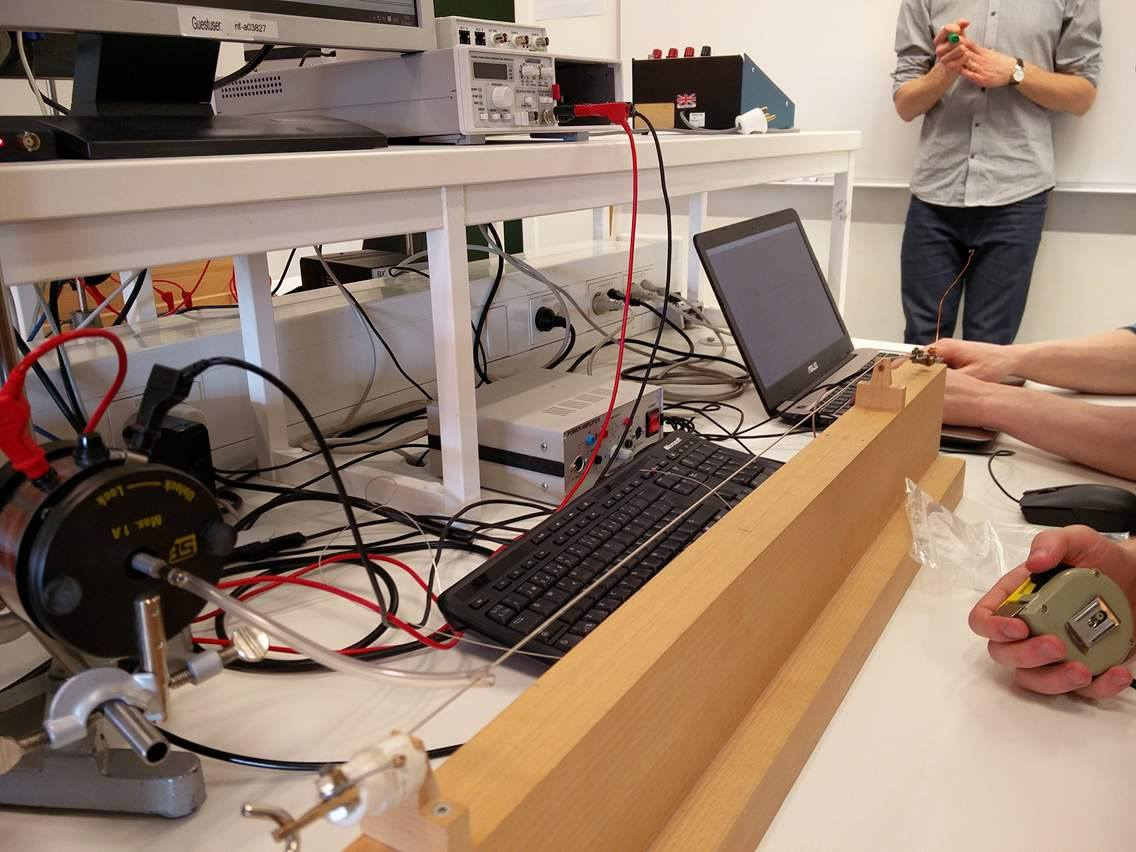
\includegraphics[width=\linewidth]{opstilling.jpg}
    \caption{Billedet af forsøget.}
    \label{fig:opstilling}
\end{figure}
\end{document}
